\chapter[Majorana geometric representation...]{Majorana geometric representation of permutation symmetric pure multiqubit states}\label{chap29} 

\renewcommand{\thefootnote}{\fnsymbol{footnote}}

\Authorline{Sudha,$^{1,2,}$\footnote{arss@rediffmail.com} 
A R Usha Devi,$^{3,2,}$\footnote{arutth@rediffmail.com} and 
A K Rajagopal$^{2,}$\footnote{attipat.rajagopal@gmail.com}}

\authinfo{$^{1}$Department of Physics, Kuvempu University, Shankaraghatta-577 451, India.\\
$^{2}$Inspire Institute Inc., Alexandria, Virginia 22303, USA.\\
$^{3}$Department of Physics, Bangalore University, Bangalore-560 056, India.} 

\begin{abstract}
This article presents an overview of the Majorana geometric representation of permutation symmetric  pure multiqubit states and its significance in quantum information processing. As early as 1932, Majorana had proposed that a pure permutation symmetric state of $N$ spin-$\frac{1}{2}$ particles can be represented by $N$ spinors, which correspond geometrically to $N$ points on the Bloch sphere. A novel use of the Majorana geometric
representation leads  to the classification of entanglement families of permutation symmetric qubits -- based on the number of distinct  spinors  and their arrangement in constituting the multiqubit state. The Majorana classification offers an elegant approach to investigate how correlation information of the {\em whole}  pure symmetric state gets imprinted in its {\em parts}. As an example, we show that the correlation information of pure symmetric three-qubit states with two distinct Majorana spinors is completely determined by their two-qubit marginals. We explicitly determine the {\emph {three}} distinct spinors characterizing the three-qubit GHZ state and the superposition of W, and its obverse state $\bar W$. While the GHZ state cannot be determined by its parts, we illustrate that the W$\bar W$ superposition possesses genuine three-qubit entanglement, which is robust under the loss of a qubit and is imprinted uniquely in its two-party reduced states. This example clearly brings out the contrasting correlation features of states within the same entanglement family, discerned through the celebrated Majorana geometric representation.  
\end{abstract}

\begin{center}
\textbf{\Large In memory of Professor G. Ramachandran}
\end{center}

\renewcommand{\thesection}{\Roman{section}}
\section{Introduction}\label{chap29-sec1}

Multiqubit states that are invariant under exchange of any pair of particles form an important class among quantum states due to their experimental significance and mathematical elegance \cite{sym1,sym1a,sym1b,sym2,sym3}. The class of symmetric states comprises of the well-known Greenberger-Horne-Zeilinger(GHZ) \cite{ghz}, W, and Dicke states \cite{dicke} etc. Mathematical simplicity in addressing $N$-qubit  states obeying permutation symmetry results because the states are confined to the $N+1$ dimensional subspace of the $2^N$ dimensional Hilbert space. The $N+1$ dimensional subspace is spanned by the Dicke states, $\{\vert N/2, N/2-l\rangle,  l=0,1,2,\ldots,N\}$, which are the simultaneous eigenstates of the squared collective angular momentum operator $J^2$ and its $z$-component $J_z$. An elegant geometrical representation for  multiqubit symmetric states in terms of $N$-points on the Bloch sphere $S^2$ was proposed by Majorana \cite{majorana} as early as 1932. The geometric representation of multiqubit states based on their characteristic $N$-qubits (spinors), the so-called {\em Majorana geometric representation} for symmetric states \cite{majorana,1945,makela} has been  immensely useful in diverse branches of physics \cite{1945,jpa4,arxiv4,jpa5,ejtp6} in general and in quantum information science \cite{solano, mixed, usa, usa1,usa2,usa3,markham1,markham2,gebastin,markham3} in particular.  The significance of Majorana geometric representation in characterizing entanglement in multiqubit symmetric states has been realized in several fields and the avenues appear to be expanding. While the SLOCC classification of symmetric states in terms of the distinct spinors characterizing the state has been accomplished using the Majorana geometric representation \cite{solano, mixed}, it is shown that the reducibility/irreducibility features of multiparty correlations in several important classes of states can also be captured \cite{usa1,usa2,usa}. 

Understanding different kinds of correlations exhibited by multiparticle quantum systems is one of the  central issues of importance in quantum information science \cite{Niel}. Two $N$-party {\em pure} states $\vert\phi\rangle$, $\vert \psi\rangle$  can be obtained from one another by means of stochastic local operations and classical communications (SLOCC)  if and only if there exists an invertible local operation (ILO) \cite{Dur} $A_1\otimes A_2\otimes \cdots \otimes A_N$ such that $\vert \phi\rangle=\left(A_1\otimes A_2\otimes \cdots \otimes A_N\right)\vert\psi\rangle$. General classification of distinct kinds of entanglement that are inequivalent under SLOCC has gained considerable attention \cite{Dur,Ver,Lamata}. It is convenient to address this issue by restricting to special classes of states exhibiting some particular symmetry, in order to tackle the algebraic complexity associated with exponentially increasing size of the Hilbert space. In the important case of  $N$-qubits obeying permutation symmetry, it is sufficient to search for identical ILOs of the form $A\otimes A\otimes\cdots \otimes A$ to verify the SLOCC equivalence of two pure states \cite{solano,bastin}. The significance of such considerations is catching up and  innovative experimental schemes to generate a large variety of multiqubit states has been proposed \cite{newexpt1,newexpt2}. The geometric representation proposed by Majorana \cite{majorana} offers a deeper understanding on how different entanglement families emerge, depending on the number and arrangement of the independent spinors (qubits) constituting the {\em pure} symmetric state \cite{solano}. 

Determining if higher order correlations follow entirely from lower order ones is also a question of fundamental interest both from the modern perspective of quantum information science \cite{SP1,SP2,SP2b} as well as in many body physics \cite{Coleman}. Linden, Popescu and Wootters \cite{SP1,SP2,SP2b} proved that the correlation content of {\em almost all} pure states, shared by $N$ parties, is already contained in their reduced states i.e., the higher order correlations are uniquely determined by lower order ones \cite{SP1,SP2,SP2b}. In this article, we discuss the ``whole and its parts" issue for three-qubit pure symmetric states belonging to two SLOCC inequivalent families, the class of states with two distinct Majorana spinors and the ones with three distinct spinors. More specifically, we address the question ``{\em Is there any intrinsic connection between SLOCC classification of pure states with their determinability in terms of reduced subsystems?}". We show that not all states that are interconvertible into one another through SLOCC operations exhibit the same reducibility/irreducibility of correlations. This has been accomplished by considering three-qubit GHZ state and superposition of W and its obverse state $\bar{W}$, both belonging to the same SLOCC family containing three distinct spinors.   We also demonstrate that two-qubit reduced density matrices uniquely determine the family of three-qubit  pure symmetric states comprised of two distinct Majorana spinors, the so-called {\emph {Dicke class of states}}.

\section{Majorana geometric representation of permutation symmetric multiqubit pure states}\label{chap29-secII} 

In his 1932 paper \cite{majorana} Majorana proposed that a pure spin $j=\frac{N}{2}$ quantum state can essentially be represented as a {\em symmetrized} combination of $N$ constituent spinors as follows:  
\begin{equation}
\vert \Psi^{(N)}_{\rm sym}\rangle={\cal N}_N\, \sum_{P}\, \hat{P}\, \{\vert \epsilon_1, \epsilon_2, \ldots  \epsilon_N \rangle\}, \label{Maj}
\end{equation} 

\vskip -.5cm

\noindent
where 
\begin{equation}
\vert\epsilon_l\rangle= \cos(\beta_l/2)\, e^{-i\alpha_l/2}\, \vert 0\rangle +\sin(\beta_l/2)\, e^{i\alpha_l/2} \, \vert 1\rangle,\ \ l=0,1,2,\ldots, N,\label{spinor}
\end{equation}
denote the spinors constituting the symmetric state $\vert \Psi^{(N)}_{\rm sym}\rangle$; $\hat{P}$ corresponds to the set of all $N!$ permutations of the spinors (qubits) and ${\cal N}_N$ corresponds to an overall normalization factor. For example, two and three-qubit symmetric pure states have the following representations in terms of the Majorana spinors:
\begin{align*}
\vert \Psi^{(2)}_{\rm sym}\rangle &={\cal N}_2\,  \left(\vert \epsilon_1, 
 \epsilon_2\rangle+  \vert \epsilon_2,\epsilon_1\rangle\right)\\
\vert \Psi^{(3)}_{\rm sym}\rangle &={\cal N}_3\,\left(  \vert \epsilon_1,
 \epsilon_2, \epsilon_3\rangle+  \vert \epsilon_3,\epsilon_1, \epsilon_2\rangle  + \vert \epsilon_2, 
 \epsilon_3, \epsilon_1\rangle +\vert \epsilon_2,\epsilon_1,\epsilon_3\rangle\right.\\
&\quad\left. + \vert \epsilon_3,\epsilon_2,\epsilon_1\rangle+ \vert \epsilon_1, \epsilon_3, \epsilon_2\rangle \right).
\end{align*}
Eq.\ \eqref{Maj} corresponds to the {\em Majorana geometric representation} of an arbitrary symmetric state $\vert \Psi^{(N)}_{\rm sym}\rangle$ of $N$ qubits in terms of the constituent spinors $\vert \epsilon_l \rangle,\  l=1,2,\ldots N$. These spinors (qubits) correspond geometrically to $N$ points on the  Bloch sphere $S^2$ \cite{makela,jpa4,markham1,markham2,gebastin, markham3} -- with the pair of angles $(\alpha_l,\beta_l)$ determining the orientation of each point on $S^2$.

On the other hand, states of $N$-qubits obeying exchange symmetry get restricted to a $(N+1)$ dimensional Hilbert space spanned by the collective basis vectors $\left\{\left\vert \frac{N}{2}, l-\frac{N}{2}\right\rangle, l=0,1,2,\ldots N \right\}$ where,
\begin{equation}
\left\vert \frac{N}{2}, l-\frac{N}{2}\right\rangle =\frac{1}{\sqrt{^N C_l}}\,[\vert \underbrace{0, 0, \ldots}_{l}, 
\underbrace{1, 1, \ldots}_{N-l}\rangle +\ {\rm Permutations}\ ] \label{Dicke} 
\end{equation}
are the $N+1$ Dicke  states -- expressed in the standard qubit basis $\vert 0\rangle,\ \vert 1\rangle$ and $^N C_l=\frac{N!}{l!\,(N-l)!}$ denotes the binomial coefficient. An arbitrary pure symmetric state of $N$ qubits obeying exchange symmetry may thus be expressed as,    
\begin{equation}
\vert \Psi^{(N)}_{\rm sym}\rangle =\sum_{l=0}^{N}\, c_l\, \left\vert \frac{N}{2}, l-\frac{N}{2}\right\rangle,\label{sympure1}
\end{equation}
and is completely specified by the $(N+1)$ complex coefficients $c_l$.  Eliminating an overall phase and normalizing  the state  implies that $N$ complex parameters are required to completely characterize a pure symmetric state \eqref{sympure1} of $N$ qubits. While \eqref{sympure1} offers a suitable parametrization of the symmetric multiqubit system in terms of the collective parameters $c_l$, the Majorana geometric representation \eqref{Maj} leads to an intrinsic geometric picture of the  system in terms of $N$-points on the Bloch sphere $S^2$.  

The equivalence between the parameters $c_l$ of the collective representation \eqref{sympure1} and that of  the Majorana geometric representation \eqref{Maj} can be established in an elegant manner \cite{usa1,usa2,usa} as detailed in the following. 
\begin{enumerate}
\item A symmetric pure state is transformed into another symmetric pure state under identical rotations $R\otimes R\otimes \cdots \otimes R$ on all the spinors of \eqref{Maj} (which corresponds  to an equivalent collective rotation ${\cal R}$ on the state \eqref{sympure1} in the $(N+1)$ dimensional symmetric sub-space). 

\item Under identical rotation through $R^{-1}(\alpha_s,\beta_s,0)\otimes R^{-1}(\alpha_s,\beta_s,0)\otimes \cdots  $, where $\alpha_s, \beta_s$ correspond to the orientation of any one of the spinors in \eqref{Maj}, it may be identified that 
\begin{equation}
\langle 1,1\ldots , 1\vert R^{-1}(\alpha_s,\beta_s,0)\otimes R^{-1}(\alpha_s,\beta_s,0)\otimes 
\cdots   \vert \Psi^{(N)}_{\rm sym}\rangle\equiv 0.\label{rl}
\end{equation}
This is because the rotation $R_s^{-1}\otimes R_s^{-1}\cdots \otimes R_s^{-1}$ takes one of the spinors $\vert \epsilon_s\rangle$ with orientation angles $(\alpha_s, \beta_s)$ to $\vert 0\rangle$ i.e., it aligns the spinor $\vert \epsilon_s\rangle$ in the positive $z$-direction. Then, every   term in the  superposition \eqref{Maj} of the rotated state has atleast one $\vert 0\rangle$ and so, the projection $\langle 1,1,\ldots, 1\vert R_s^{-1}\otimes R_s^{-1}\otimes \cdots R_s^{-1}\vert \Psi^{(N)}_{\rm Sym}\rangle$ of the rotated state in the `all-down' direction vanishes. 

\item Eq.~\eqref{rl} holds good for  collective rotations ${\cal R}_s^{-1}=R^{-1}_s\otimes R^{-1}_s\otimes\cdots\otimes R^{-1}_s,\ \ s=1,2,\ldots, N,$ which orient {\em any} one of the constituent spinors $\vert\epsilon_s\rangle$ in the positive $z$-direction. In other words, there exist $N$ rotations $R^{-1}_s=R^{-1}(\alpha_s,\beta_s,0), s=1,2,\ldots , N$ -- in general -- which lead to the same result  \eqref{rl}.

\item In terms of the alternate representation \eqref{sympure1} of the symmetric state $\vert \Psi^{(N)}_{\rm sym}\rangle$, \eqref{rl} leads to 
{\fontsize{8pt}{10pt}\selectfont
\begin{align}
&\left\langle \frac{N}{2},-\frac{N}{2}\left\vert R^{-1}(\alpha_s,\beta_s,0)\otimes R^{-1}(\alpha_s,\beta_s,0)\otimes \cdots  \otimes R^{-1}(\alpha_s,\beta_s,0) \right \vert \Psi_{\rm sym}\right\rangle=0\nonumber \\ 
&\Rightarrow\ \ \left\langle \frac{N}{2},-\frac{N}{2}\left \vert {\cal R}_s^{-1}(\alpha_s,\beta_s,0) \left\{\sum_{l=0}^N\, c_l\, \right \vert \frac{N}{2},l-\frac{N}{2}\right \rangle\right\}=0 \nonumber \\
&{\rm i.e.,} \ \ \ \sum_{l=0}^N\, c_l\, D^{N/2*}_{l-N/2,-N/2}(\alpha_s,\beta_s,0) =0, \label{prelim}
\end{align}}\relax
where we have denoted 
$$R^{-1}(\alpha_s,\beta_s,0)\otimes R^{-1}(\alpha_s,\beta_s,0)\otimes \cdots  \otimes R^{-1}(\alpha_s,\beta_s,0)~=~{\cal R}^{-1}_s(\alpha_s,\beta_s,0)$$ 
in the collective $(N+1)$ dimensional symmetric subspace of $N$ qubits and 
$$
D^{N/2\dag}_{-N/2,\, l-N/2}=\langle N/2,-N/2\vert{\cal R}^{-1}_l \vert N/2,l-N/2\rangle,
$$
represents the collective rotation in the Wigner-$D$ representation \cite{Rose}. Substituting the explicit form of the $D$-matrix \cite{Rose}, i.e.,
{\fontsize{9pt}{11pt}\selectfont
\begin{align}
\left[D^{\frac{N}{2}\dag}(\alpha,\beta,0)\right]_{-\frac{N}{2},l-\frac{N}{2}}&= D^{\frac{N}{2}*}_{l-\frac{N}{2},-\frac{N}{2}}(\alpha,\beta,0) \nonumber\\ 
&=  \sqrt{^N\,C_l}\, \left[\cos\left(\frac{\beta}{2}\right)\right]^{N-l}\, \left[-\sin\left(\frac{\beta}{2}\right)\right]^{l} \, e^{i(l-\frac{N}{2})\alpha},\label{dmatrix}
\end{align}}\relax
and on subsequent simplification we obtain,
\begin{equation}
{\cal A}\, \sum_{l=0}^N (-1)^l\,\sqrt{^N\, C_l}\,  c_l\,  \, z^{l}=0  \label{cmj02}
\end{equation} 
where $z=\tan\left(\frac{\beta}{2}\right)\,e^{i\, \alpha}$ and the overall coefficient 
$${\cal A}=\cos^N\left(\frac{\beta}{2}\right)\,e^{-i\frac{N\,\alpha}{2}}.$$ 

In other words, the $N$ roots $z_l=\tan\left(\frac{\beta_l}{2}\right)\,e^{i\, \alpha_l}, l=1,2,\ldots N$ of the Majorana polynomial $P(z)$
\begin{equation} 
P(z)=\sum_{l=0}^N\, (-1)^l\, \sqrt{^N\, C_l}\,  c_l\,  \, z^{l}\label{Mp}
\end{equation}
determine the orientations $(\alpha_l,\beta_l)$ of the  spinors constituting the  $N$-qubit symmetric state, in terms of the collective parameters $c_l$.
\end{enumerate}

When some of the coefficients $c_l,\ r< l\leq N$ in $\vert \Psi^{(N)}_{\rm sym}\rangle$ (See~\eqref{sympure1}) are zero, its Majorana Polynomial $P(z)$ is of degree $r<N$ and the orientations of all the $N$ constituent spinors may not be determined. To see this, let us consider the example of Dicke states \eqref{Dicke}. We have only one of the coefficients non-zero i.e., $c_l=\delta_{l,r}$.  The corresponding Majorana polynomial $P(z)$ reduces to  $P(z)=(-1)^r\, \sqrt{^N\, C_r}\, z^{r}$. The $r$-fold degenerate root  $z=0$ of the polynomial leads to the specification of the spinor orientation angles $\beta_l=0,\ \ \alpha_l=$arbitrary, $l=1,2,\ldots, r$ -- leading to the identification $\vert\epsilon_l\rangle\sim \vert 0\rangle,\ l=1,2,\ldots r$ (up to an overall phase) of the constituent spinors. There is no further information about the remaining $N-r$ spinors constituting the state in terms of the Majorana Polynomial \eqref{Mp}.  It is convenient to recast the  polynomial in terms of $z'=\frac{1}{z}=\cot \left(\frac{\beta_l}{2}\right)\,e^{-i\alpha_l}$ and following the same procedure outlined above, we obtain
\begin{equation}
{\cal A'}\  \sum_{l=0}^N (-1)^l\,\sqrt{^N\, C_l}\,  c_{\frac{N}{2}-l}\,  \, z'^{N-l}=0,\label{cmj03}  
\end{equation} 
where  ${\cal A'}=\sin^N\left(\frac{\beta_l}{2}\right)\,e^{i\alpha_l\, N/2}.$ We thus obtain, 
\begin{equation} 
P(z')=\sum_{l=0}^N\, (-1)^{N-l}\, \sqrt{^N\, C_l}\,  c_l\,  \, z'^{N-l}.\label{Mp2}
\end{equation}
The $N-r$ roots of the  polynomial \eqref{Mp2} determine the orientations of the remaining $N-r$ spinors $\vert\epsilon_l\rangle$, $l=r+1,\,r+2,\,\ldots N$, constituting the state $\vert \Psi^{(N)}_{\rm sym}\rangle$. In particular, for Dicke states $\left\vert \frac{N}{2},r-\frac{N}{2}\right\rangle$, it is easy to see that \eqref{Mp2} leads to $(N-r)$-fold degenerate root $z'=0$ which corresponds to $\beta_l=\pi/2,\ \alpha_l=$ arbitrary i.e., $\vert \epsilon_l \rangle \equiv \vert 1 \rangle$, $l=r+1,\,r+2,\, \ldots N$. It may be readily seen that except for the  {\em all-up} ({\em all down}) $N$-qubit Dicke states 
$$\left\vert \frac{N}{2}, \frac{N}{2}\right\rangle\equiv \vert 0,\,0,\ldots,0\rangle\left(\left\vert \frac{N}{2},-\frac{N}{2}\right\rangle\equiv \vert 1,\,1,\ldots,1 \rangle\right),$$ 
for which the Majorana Polynomial  $P(z)=(-1)^N\, z^N$ ($\ P(z')=(-1)^N z'^{N}$) results in $N$-fold degenerate root, all the other  Dicke states $\left\vert \frac{N}{2},l-\frac{N}{2}\right\rangle,\break l\neq 0, N$ are characterized by two distinct spinors, $\vert 0\rangle$, $\vert 1 \rangle$ each occurring $r$ and $N-r$ times respectively. 

The GHZ state $\frac{1}{\sqrt{2}}\left[\left\vert \frac{N}{2},\frac{N}{2}\right\rangle+ \left\vert \frac{N}{2},-\frac{N}{2}\right\rangle\right]$ of $N$ qubits  satisfy the polynomial equation $1 +(-1)^N\, z^{N}=0$, solutions of which are  $N^{\rm th}$ roots of unity (when $N$ is odd) $z_{l}=e^{\frac{2\pi\, i\, l}{N}};\ l=0,1,2,\ldots N-1$ (when $N$=even, we have $z_{l}=e^{\frac{2\pi\, i}{N}(l-\frac{1}{2})}$). The associated  Majorana spinors are given by, $\vert \epsilon_{l}\rangle=\sqrt{\frac{z_l}{2}}\left[ \vert 0\rangle + z_l \vert 1\rangle\right]$, $l=0,1,2,\ldots, N-1.$ 

We list some examples of   symmetric states of two and three qubits and the corresponding constituent spinors in Table.~\ref{chap29-tab1}. 
\vskip -8pt

\counterwithout{table}{chapter}
{\tabcolsep=0pt
\setcounter{table}{0}
\scriptsize\begin{longtable}{@{}|c@{\hspace{-.2cm}}c|@{\,}c@{\,}|@{\,}c@{\,}|@{\;}c@{\,}|@{}}
\caption{Majorana spinors for some two and three-qubit symmetric states}\label{chap29-tab1}\\
\hline
& $\begin{array}{c@{\,}} {\rm Symmetric\ state} \\ {\rm in\ the} \\ {\rm collective\ basis}\\ \left\vert\frac{N}{2},l-\frac{N}{2}\right\rangle \end{array}$ & $\begin{array}{c}{\rm Polynomial equation}\\ {\rm and its solutions} \end{array}$ & Majorana spinors & $\begin{array}{c} {\rm Symmetrization\ of}\\ {\rm Majorana\ spinors}\\ {\rm as\ in\ Eq.~\eqref{Maj}} \\  ({\rm expressed\ in\ the}\\ {\rm standard\ qubit\ basis})\end{array}$\\
\hline 
N=2; &  $\frac{\vert 1,1\rangle + \vert 1,-1\rangle}{\sqrt{2}}$
    & $\begin{array}{c} 1+ z^2=0, \\ z_{1,2}=e^{\pm i\frac{\pi}{2}};\\ \beta_{1,2}=\frac{\pi}{2}; \alpha_{1,2}=\pm\frac{\pi}{2}\end{array}$
    & $\begin{array}{c} \vert \epsilon_{1}\rangle= \frac{e^{-i\frac{\pi}{4}}}{\sqrt{2}}\left(\vert0\rangle+  i \vert 1\rangle\right) \\  \\ \vert \epsilon_{2}\rangle=
  \frac{e^{i\frac{\pi}{4}}}{\sqrt{2}}\left(\vert0\rangle-  i \vert 1\rangle\right)\end{array}$ & $\frac{\vert 0,0\rangle + \vert 1,1\rangle}{\sqrt{2}}$ \\
\hline 
& $\frac{\vert 1,1\rangle - \vert 1,-1\rangle}{\sqrt{2}}$
& $\begin{array}{c} z^2-1=0,\\ z_{1,2}=\pm 1; \beta_{1,2}=\pm \frac{\pi}{2}; \\ 
\alpha_{1,2}=0 \end{array}$ & $\begin{array}{c}\vert \epsilon_{1}\rangle=
  \frac{1}{\sqrt{2}}\, \left(\vert 0\rangle+ \vert 1\rangle\right)  \\ 
   \vert \epsilon_{2}\rangle=
  \frac{1}{\sqrt{2}}\, \left(\vert0\rangle- \vert 1\rangle\right)
  \end{array}$  & $\frac{\vert 0,0\rangle - \vert 1,1\rangle}{\sqrt{2}}$\\        
\hline 
& $\vert 1,0\rangle $
& $\begin{array}{c} z=0,\ \ z^{-1}=0  \\ z_{1}=0, z_2=z^{-1}=0 \\  \beta_{1,2}=0, \pi;\\ \alpha_{1,2}={\rm arbitrary}\end{array}$
 & $\begin{array}{c}\vert \epsilon_{1}\rangle=\vert0\rangle \\ 
\vert \epsilon_{2}\rangle=
  \vert1\rangle \end{array}$ & $\frac{\vert 0,1\rangle + \vert 1,0\rangle}{\sqrt{2}}$\\        
\hline 
N=3;  
&  $\frac{\left\vert \frac{3}{2},\frac{3}{2}\right\rangle+\left\vert \frac{3}{2},-\frac{3}{2}\right\rangle}{\sqrt{2}}$
& $\begin{array}{c} 1- z^3=0, \\ z_{r}=e^{\frac{2\pi\, i\, r}{3}},   \\ \beta_{r}=\frac{\pi}{2}; \alpha_{r}=\frac{2\pi\, r}{3},\\ r=0,1,2.\end{array}$
& $\begin{array}{@{}c@{}}\vert \epsilon_{r}\rangle=  \sqrt{\frac{z_r}{2}}\, \left(\vert 0\rangle+ z_r\, \vert 1\rangle\right),  \\ \ r=0,1,2\end{array}$
& $\frac{\vert 0,0,0\rangle+\vert 1,1,1\rangle}{2}$ \\
\hline 
& $\frac{\left\vert \frac{3}{2},\frac{3}{2}\right\rangle-\left\vert \frac{3}{2},-\frac{3}{2}\right\rangle}{\sqrt{2}}$
& $\begin{array}{@{}c@{}}z^3+1=0, \\ 
z_{r}=e^{\frac{2\pi\, i\,}{3}(r-\frac{1}{2})} \\
\beta_{r}=\frac{\pi}{2}; \alpha_{r}=\frac{2\pi}{3}(r-\frac{1}{2}),\\ r=0,1,2 \end{array}$
& 
$\begin{array}{@{}c@{}}\vert \epsilon_{r}\rangle=  \sqrt{\frac{z_r}{2}}\, \left(\vert0\rangle+z_r\, \vert 1\rangle\right),  \\ \ r=0,1,2\end{array}$
  & $\frac{\vert 0,0,0\rangle - \vert 1,1,1\rangle}{2}$
  \\ 
\hline
& $\frac{\left\vert \frac{3}{2},\frac{1}{2}\right\rangle\pm \left\vert \frac{3}{2},-\frac{1}{2}\right\rangle}{\sqrt{2}}$
& $\begin{array}{@{}c@{}} z^2\mp z=0\\  
z_{1}=\pm 1, z_2=0, z_3^{-1}=0;\\
\beta_{1}=\pm \frac{\pi}{2};\, \alpha_1=\mp\pi;\\ \beta_{2}=0; \beta_3=\pi.\end{array}$
& $\begin{array}{c}\vert \epsilon_{1}\rangle=
  \frac{1}{\sqrt{2}}\left(\vert 0\rangle \pm \vert 1\rangle\right),  
 \\  \vert \epsilon_{2}\rangle=\vert 0\rangle, \ 
 \vert \epsilon_{3}\rangle=\vert 1\rangle\end{array} $ 
 & $\begin{array}{@{\,}l@{\,}}
\frac{1}{\sqrt{6}}\, [\vert 0,0,1\rangle+\vert 0,1,0\rangle \\ 
+\vert 0,0,1\rangle 
 \pm \vert 0,1,1\rangle\\ 
 \pm \vert 1,0,1\rangle\pm \vert 1,1,0\rangle]
 \end{array}$  \\       
  \hline
& $\left\vert \frac{3}{2}, -\frac{1}{2}\right\rangle$
& $\begin{array}{c} z=0, z^{-2}=0 \\
z_{1}=0,z_2^{-1}=z_3^{-1}=0,\\   \beta_{1}=0, \beta_{2,3}=\pi \\ \alpha_{1,2,3}={\rm arbitrary}, \end{array} $
& $\vert \epsilon_{1}\rangle=\vert0\rangle, \ \vert \epsilon_{2,3}\rangle=\vert 1\rangle$ 
 & $\begin{array}{@{\,}l@{\,}}\frac{1}{\sqrt{3}}\, [\vert 0,1,1\rangle+\vert 1,1,0\rangle\\ +\vert 1,0,1\rangle]\end{array}$\\
 \hline        
\end{longtable}}
\bigskip

\section{SLOCC classification of multiqubit symmetric states}\label{classification}

Multiparticle entanglement  can be of different kinds \cite{Dur}. Two multiparty states have the same kind of entanglement if they can be obtained from each other other via SLOCC with nonzero probability. It is well-known that three-qubit GHZ and W states are inequivalent under SLOCC and are representatives of inequivalent three-party entanglement. Understanding  inequivalent classes of multiparticle entanglement, which are not interconvertible into each other under SLOCC operations is of fundamental importance \cite{Dur,Ver,Lamata,solano}. In the following, we outline \cite{solano} the SLOCC classification of pure symmetric multiqubit states based on Majorana geometric representation.

As we have noted in Sec.~II,  the roots of the Majorana polynomial (\ref{Mp}) (and (\ref{Mp2})) could be degenerate  and hence not all the  $N$ constituent spinors of a pure symmetric $N$ qubit state are distinct. Let $\vert \epsilon_1\rangle, \vert \epsilon_2\rangle,\ldots, \vert \epsilon_d\rangle,\ d\leq N$ be the number of distinct spinors, in a $N$ qubit pure symmetric state (\ref{Maj}).  Then, the list of numbers 
$$
\left\{n_1,\,n_2,\ldots ,n_d;\ \ n_1\geq n_2\geq\cdots \geq n_d; \ \  n_1+n_2+\cdots+n_d=N\right\}
$$ 
corresponds respectively to the number of times the independent spinors $\vert\epsilon_i\rangle$, ($i=1,2,\ldots d\leq N$) appear in the symmetric state (\ref{Maj}) under consideration. The number $d\leq N$, called the {\em diversity degree} and the list of numbers $\left\{n_1,\,n_2,\ldots ,n_d;\  n_1\geq n_2\geq \cdots n_d,\  \sum_{i=1}^{d} n_i=N\right\}$, called the {\em degeneracy configuration}, form the key elements in the classification of  pure symmetric states \cite{solano}. The different classes  (based on the number of distinct spinors and their arrangement in a given $N$-qubit symmetric state)  are denoted by $\{{\cal D}_{n_1,n_2,\ldots n_d}\}$. An identical ILO $A^{\otimes N}$ transforms a symmetric state belonging to the class $\{ {\cal D}_{n_1,\,n_2,\ldots, n_d}\}$ to another state of the {\em same} class. More explicitly, we have 
\begin{equation}
\vert D_{n_1,n_2\ldots, n_d}\rangle \ \stackrel{\rm  ILO}{\longrightarrow}\ \vert D'_{n_1,\,n_2\ldots, n_d}\rangle={A}^{\otimes N}\,\vert D_{n_1,n_2\ldots, n_d}\rangle\label{chap29-eq12}
\end{equation}  
with the constituent spinors transforming as 
$\vert\epsilon'_i\rangle~=~A\, \vert\epsilon_i\rangle$, $i=1,2,\ldots d$. This forms the main basis of the SLOCC classification of symmetric pure 
states \cite{solano}. 
\begin{enumerate}
\item $\{{\cal D}_N\}$: When all the $N$ solutions of the Majorana polynomial are identically equal, the corresponding class of  symmetric states is given by 
\begin{equation}
\vert D_N\rangle=\vert \epsilon,\epsilon,\ldots \epsilon\rangle,
\end{equation} 
where the diversity degree  $d=1$; the states belonging to this family of separable symmetric states  is denoted by $\vert D_N \rangle$.  

\item $\{{\cal D}_{n_1,n_2};\ n_1=N-k,\ n_2=k=1,2,\ldots, [N/2]\}$: The  states with two distinct spinors have the form, 
\begin{equation}
\vert D_{N-k,k}\rangle={\cal N}\,[\vert \underbrace{\epsilon_1, \epsilon_1,\ldots \epsilon_1}_{N-k}, \underbrace{\epsilon_2, \epsilon_2,\ldots \epsilon_2}_{k}\rangle+{\rm  Permutations}]\label{n1n2}
\end{equation} 
where $k=1,2, \ldots [N/2]$.  

Dicke states $\left\vert \frac{N}{2}, k-\frac{N}{2}\right\rangle$ are the representative states of the entanglement class $\{{\cal D}_{N-k,k}\}$ with two independent spinors  and clearly, they are all inequivalent under  SLOCC (as the degeneracy classification  is different for each $k=1,2, \ldots [N/2]$).

\item $\{{\cal D}_{1,1,\ldots, 1}\}$:  When the $N$ roots of the Majorana Polynomial \eqref{Maj} are all distinct, the pure symmetric states constitute  the class\break $\lbrace {\cal D}_{1,1,1,\ldots,1}\rbrace$ with diversity degree  $d=N$. Clearly, the $N$ qubit GHZ state is a representative of this entanglement class. 
\end{enumerate}
The number of SLOCC classes  grows  with the increase in the number of qubits: For $N=2$, there are only $2$ entanglement families given by 
$D_{2}$ (the separable class) and $D_{1,\,1}$; for $N=3$ there are $3$ SLOCC classes given by $D_{3}$, $D_{2,\,1}$ and $D_{1,\,1,\,1} $ etc.  In general, the number of entanglement families for a symmetric $N$-qubit state grows \cite{solano}, based entirely on the partition of the number $N$ in the arrangement 
$$\left\{n_1,\,n_2,\ldots ,n_d; n_1\geq n_2\geq\cdots\geq n_d;\   \sum_{i=1}^{d} n_i=N\right\}.$$ 
However, the Majorana classes  with diversity degree $d\geq 4$ contain a continuous range of SLOCC classes, depending on a continuous  parameter and the states with different value of this continuous  parameter  are not SLOCC convertible into each other \cite{solano}. 

  
\section{Determining the Whole pure state from its parts}\label{chap29-eqIV} 

While the equivalence of quantum states under SLOCC is known to indicate that states belonging to the same equivalence class can be used to implement similar quantum information tasks \cite{Dur}, we address the question "{\emph{Do the {\rm SLOCC} interconvertible symmetric pure states possess similar irreducibility features?}}" by considering specific example of three-qubit symmetric states belonging to the same SLOCC class $\{{\cal D}_{1,1,1}\}$.  With the help of this example, we demonstrate explicitly that the states of the same Majorana class could exhibit contrasting irreducibility features. In fact, we show that three-qubit GHZ state and its local unitary equivalent states are the only ones of the Majorana class $\{{\cal D}_{1,1,1}\}$,  which are undetermined by their two-qubit reduced systems \cite{SP1,Walck,Walck2}. 

\subsection*{A. Irreducibility features of three-qubit symmetric states of the class $\{{\cal D}_{1,1,1} \}$:}

We consider two specific examples of the SLOCC family $\{{\cal D}_{1,1,1}\}$,  the first being the three-qubit 
GHZ state,  
\begin{equation}
\vert {\rm GHZ}\rangle= \frac{1}{\sqrt{2}}\, [\vert 0,0,0\rangle +  \vert 1,1,1\rangle].\label{GHZ}
\end{equation}      
The Majorana polynomial equation \eqref{Maj} for this state has a simple structure $1-z^3=0$, solutions of which are cube roots of unity $\omega$, $\omega^2$, $\omega^3=1$ and the corresponding spinors constituting the state are readily identified to be 
\begin{equation}
\vert \epsilon_1\rangle =\frac{1}{\sqrt{2}}[\vert 0\rangle+\omega\, \vert 1\rangle],\ \  \vert \epsilon_2\rangle =\frac{1}{\sqrt{2}}[\vert 0\rangle+\omega^2\, \vert 1\rangle], \ \ \vert \epsilon_3\rangle =\frac{1}{\sqrt{2}}[\vert 0\rangle+ \vert 1\rangle].\label{chap29-eq16}
\end{equation}
GHZ state is fragile under the loss of a qubit, with vanishing pairwise concurrence \cite{Wot,Wot2} for any pairs of two-qubit reduced density matrices; but it exhibits genuine three-party entanglement \cite{Dur,RaRe} with the maximum tangle  $\tau=1$ \cite{Kun}.  The state exhibits irreducible three-party correlations which can not be determined by its reduced states \cite{SP1,Walck,Walck2}. 

We consider another three-qubit state which belong to the same SLOCC class $\{{\cal D}_{1,1,1}\}$ of three distinct Majorana spinors: 
\begin{equation}
\vert \eta\rangle = \frac{1}{\sqrt{2}} [\vert {\rm W}\rangle +  \vert{\rm \bar{W}}\rangle].\label{Wsup}
\end{equation}         
This  is an equal superposition of the three-qubit W state $\vert{\rm W}\rangle=\break\frac{1}{\sqrt{3}}[\vert 0,0,1\rangle+\vert 0,1,0\rangle+\vert 1,0,0\rangle]$  
 and its obverse state $\vert{\rm \bar{W}}\rangle=\frac{1}{\sqrt{3}}[\vert 1,1,0\rangle+\vert 1,0,1\rangle+\vert 0,1,1\rangle].$ The state $\vert \eta\rangle$ has genuine three-party entanglement, quantified in terms of the tangle $\tau=1/3$, and it is also robust under the loss of qubits -- as reflected through the concurrence $C=1/3$ for any two-qubit pairs.  The three-qubit symmetric state $\vert \eta\rangle$ given by \eqref{Wsup} satisfies the Majorana polynomial equation $z(z-1)=0$  and the corresponding spinors constituting the state are 
\begin{equation}
\vert \epsilon'_1\rangle =\vert 1\rangle,\ \ \  \vert \epsilon'_2\rangle =\frac{1}{\sqrt{2}}[\vert 0\rangle+ \vert 1\rangle], \ \ \vert \epsilon'_3\rangle = \vert 0\rangle. 
\end{equation}
The states $\vert {\rm GHZ}\rangle$ and the W$\bar W$ state $\vert \eta\rangle$   can be {\em locally} converted from one another,  with the help of an identical ILO i.e.,
\begin{equation}
\vert {\rm GHZ}\rangle=\left(A\otimes A\otimes A\right) \vert \eta\rangle,\ \   \mbox{where}\ \ A=\left(\begin{array}{cc} 1 & \omega \\ 1 & \omega^2\, \end{array}\right).\label{GHZ&eta}
\end{equation}
The corresponding Majorana spinors  of the states $\vert \eta\rangle$ and $\vert{\rm GHZ}\rangle$ are  related to each other up to an overall factor: $A\, \vert\epsilon_1'\rangle=\sqrt{2}\omega\, \vert\epsilon_1\rangle$, $A\, \vert\epsilon_2'\rangle=-\omega^2\, \vert\epsilon_2\rangle$, and $A\, \vert\epsilon_3'\rangle=   \sqrt{2}\,  \vert\epsilon_3\rangle$. We now exhibit how the higher order correlation in  the W$\bar W$ superposition state $\vert \eta\rangle$ is imprinted in its two-qubit reduced states \cite{SP1,usa,usa1,usa2}. 

Let us suppose that a mixed  three-qubit state $\hat\gamma$ too has the same two-qubit reduced system $\varrho_{12}$, as that of the W$\bar W$ superposition state $\vert \eta\rangle.$ Denoting the pure state $\vert \Gamma\rangle$ to be containing the three qubits and the environment such that  
\[ 
{\rm Tr}_{E}[\vert\Gamma\rangle\langle \Gamma\vert]=\hat\gamma,
\] 
the two-party reduced state $\varrho_{12}$ can be expressed as 
$$
\varrho_{12}={\rm Tr}_{3, E}[\vert \Gamma\rangle\langle \Gamma\vert].
$$ 
The two-qubit reduced system $\varrho_{12}$ of the pure state $\vert\eta\rangle$ is a rank-2 state given by,  
\begin{align*}
& \varrho_{12}=\vert \chi_0\rangle\langle \chi_0\vert + 
\vert \chi_1\rangle\langle \chi_1\vert, \ \ \ \mbox{where}\label{ws2}\\ 
& \vert \chi_0\rangle=\frac{1}{\sqrt{6}}[|1,0\rangle+|0,1\rangle+|1,1\rangle], \ \ \vert \chi_1\rangle=\frac{1}{\sqrt{6}}[|0,0\rangle+|0,1\rangle+|1,0\rangle].  \nonumber
\end{align*}
Given that the two-party reduced state $\hat{\varrho}_{12}$ also belongs to the extended pure state $\vert\Gamma\rangle$ (and in turn to the mixed state $\hat\gamma$) of the three qubits and the environment, we must have  
\begin{equation}
\vert\Gamma\rangle=\vert \chi_0\rangle\vert E_0\rangle +\vert \chi_1\rangle\vert E_1\rangle, \ \ \ \langle E_i\vert E_j\rangle=\delta_{i,j},\label{ws3}
 \end{equation}     
In terms of the basis states of qubit 3, the states of the environment $\vert E_{0}\rangle, \vert E_{1}\rangle$ are given by
\begin{align*}
\vert E_0\rangle&=\vert 0\rangle\,  \vert e_{00}\rangle+\vert 1\rangle\,  \vert e_{01}\rangle, \nonumber\\ 
\vert E_1\rangle&=\vert 0\rangle\,  \vert e_{10}\rangle+\vert 1\rangle\,  \vert e_{11}\rangle.
\end{align*}   
Thus, \eqref{ws3} takes the following form: 
\begin{align} 
|\Gamma\rangle&=\frac{1}{\sqrt{6}}[(|1_1,0_2,0_3\rangle+|0_1,1_2,0_3\rangle+|1_1,1_2,0_3\rangle)|e_{00}\rangle\nonumber\\
&\quad +(|1,0,1\rangle+|0,1,1\rangle+|1,1,1\rangle)|e_{01}\rangle \nonumber \\
&\quad + (|0,0,0\rangle+|0,1,0\rangle+|1,0,0\rangle)|e_{10}\rangle\nonumber\\
&\quad +(|0,0,1\rangle +|0,1,1\rangle+|1,0,1\rangle)|e_{11}\rangle] \label{Gamma}
\end{align}
Now, demanding that the reduced system $\hat{\varrho}_{13}$ of $\vert \eta\rangle$ is also shared by  $\vert \Gamma\rangle$ leads to further constraints.  
\begin{enumerate}
\item First we compare  $\langle 0,1\vert \hat{\varrho}_{13}\vert 0,1\rangle$,  from the states \eqref{Wsup} and \eqref{ws3}: We have, $\langle 0,1|{\rm Tr}_{2}\,[\vert\eta\rangle \langle\eta\vert]\, |0,1\rangle= \frac{1}{3}$ and $\langle 0,1|{\rm Tr}_{2,E}\,[\vert\Gamma\rangle \langle\Gamma\vert]\, |0,1\rangle= \frac{1}{6}\langle e_{01}|e_{01}\rangle+\frac{1}{3}\langle e_{11}|e_{11}\rangle$ leading to $\langle e_{01}|e_{01}\rangle+2\langle e_{11}|e_{11}\rangle=2$. 

\item Next, we compare  $\langle 1,1\vert \hat{\varrho}_{13}\vert 1,1\rangle$ evaluated from the states $\vert\eta\rangle$ and $\vert\Gamma\rangle$: We get, $\langle 1,1|{\rm Tr}_{2, E}\, [|\Gamma\rangle \langle\Gamma|]\,\vert 1,1\rangle=\frac{1}{3}\langle e_{01}|e_{01}\rangle+\frac{1}{6}\langle e_{11}|e_{11}\rangle$ and $\langle 1,1|{\rm Tr}_{2}\, [|\eta\rangle \langle\eta|\vert\, |1,1\rangle=\frac{1}{6}$ implying, $2\langle e_{01}|e_{01}\rangle+\langle e_{11}|e_{11}\rangle=1$. From these relations we obtain $\langle e_{11}|e_{11}\rangle=1$, $\langle e_{01}|e_{01}\rangle=0$ (or $\vert e_{01}\rangle\equiv 0$). Further, from the orthonormality property $\langle E_i\vert E_j\rangle=\delta_{i,j}$ it follows that $\langle e_{00}\vert e_{00}\rangle=1,$ and $\vert e_{10}\rangle\equiv 0$. 

\item Finally, a comparison of the matrix elements 
$$\langle 0,0|{\rm Tr}_{2,E}\,[\vert\Gamma\rangle \langle\Gamma\vert]\break |0,1\rangle= \frac{1}{6}\, \langle e_{00}|e_{11}\rangle$$ and  
$$\langle 0,0|{\rm Tr}_{2}\,[\vert\eta\rangle \langle\eta\vert]\, |0,1\rangle= \frac{1}{6}$$ 
lead to 
$$\langle e_{00}|e_{11}\rangle=1 \mbox{ or } \vert e_{11}\rangle\equiv \vert e_{00}\rangle.$$ 
Thus,  the extended pure state \eqref{ws3} should take the form $\vert \Gamma\rangle\equiv \vert \eta\rangle \, \vert e_{00}\rangle$. 
\end{enumerate}
In other words,  the three-qubit pure state $\vert \eta\rangle$  is uniquely determined by its two-qubit reduced systems and is therefore, reducible. 

This illustrative example of three qubits supports the already existing general result \cite{Walck,Walck2} that only the $N$ qubit GHZ state and its local unitarily equivalents remain undetermined by their reduced density matrices. Moreover, this clearly projects out the contrasting  irreducibility features of two SLOCC interconvertible states \eqref{GHZ} and \eqref{Wsup} of the {\em same} entanglement family $\{{\cal D}_{1,1,1}\}$.   

Shruti et al., \cite{arvind} experimentally reconstructed the W$\bar W$ three-qubit state on an NMR quantum information processor of three qubits,  establishing that the correlation content of the state is indeed imprinted in  its two-party reduced density matrices. Furthermore, using an explicit measurement-based scheme (based on the local invertible transformation given in \eqref{GHZ&eta})  they filtered out the  three-qubit GHZ state from the W$\bar W$ state experimentally. This indeed has important implications that  entangled states with different correlation properties -- but  belonging to the same SLOCC class -- perform equally well in a given quantum computational task.

\subsection*{B. Irreducibility features of three-qubit symmetric states of the class $\{{\cal D}_{2,1} \}$:}

We now consider a three-qubit pure symmetric state with two of the spinors $\vert \epsilon_1\rangle,\vert \epsilon_2\rangle,$ distinct i.e., the states belonging to the SLOCC class $\{D_{2,1}\}.$  The symmetrized three-qubit state (see \eqref{Maj}) is given by,   
\begin{align}
\vert D_{2,1}\rangle&={\cal N}\, \sum_{P}\hat{P}\left\{\vert \epsilon_1, \epsilon_1, \epsilon_2\rangle\right\}\nonumber \\
&={\cal N}\,\left[ \vert \epsilon_1, \epsilon_1, \epsilon_2\rangle +\vert \epsilon_2, \epsilon_1, \epsilon_1\rangle + \vert \epsilon_1, \epsilon_2, \epsilon_1\rangle \right],\label{3qubitW}
\end{align}
where the spinors $\vert\epsilon_s\rangle= R_s\vert 0_s\rangle=\cos(\beta_s/2)\, e^{-i\alpha_s/2}\, \vert 0_s\rangle +\sin(\beta_s/2)\, e^{i\alpha_s/2}\break \vert 1_s\rangle,\ s=1,2$. We simplify (\ref{3qubitW}) as follows: 
\begin{align}
\vert D_{2,1}\rangle &= {\cal N}_3\,\left[\sum_P {\hat P}\,\{R_1\otimes R_1\otimes R_2\}\right] \vert 0_1,0_2,0_3\rangle \nonumber\\ 
&= {\cal N}_3\, \left(R_1\otimes R_1\otimes R_1\right)\, \sum_P {\hat P}\, \{I\otimes I\otimes R_{1}^{-1}R_2 \} \vert 0_1,0_2,0_3\rangle.\label{3W2}
\end{align}
Denoting $\left(R^{-1}_1\otimes R^{-1}_1\otimes R^{-1}_1\right) \vert D_{2,1}\rangle=\vert D'_{2,1}\rangle$, where $\vert D'_{2,1}\rangle$  is local unitarily related to  $\vert D_{2,1}\rangle$ and belongs to the same SLOCC class $\{D_{2,1}\}$, we get, 
\begin{equation}
\vert D'_{2,1}\rangle={\cal N}_3\,\left[ \vert 0_1,0_2,\epsilon'_2\rangle  +\vert \epsilon'_2, 0_2, 0_3\rangle + \vert 0_1,  \epsilon'_2, 0_3\rangle \right]     
\end{equation}
with $\vert\epsilon'_2\rangle=R_1^{-1}\,R_2\vert \epsilon_2\rangle=c_0\,\vert 0\rangle +\, c_1\,\vert 1\rangle$, $c_0^2+c_1^2=1.$ We thus obtain the states belonging to the class of 3-qubit symmetric pure states  $\vert D_{2,1}\rangle$, with only two distinct Majorana spinors (upto an identical local unitary transformation) as
\begin{equation}
\vert D'_{2,1}\rangle=a\vert 0_1,0_2,0_3\rangle+b[\vert 1_1,0_2,0_3\rangle +\vert 0_1,1_2,0_3\rangle+\vert 0_1,0_2,1_3\rangle]\label{Wfin}
\end{equation}
where $a=\frac{\sqrt{3}\, c_0}{\sqrt{3\vert c_0\vert^2+\vert c_1\vert^2}}$, $b=\frac{ c_1}{\sqrt{9\vert c_0\vert^2+3\vert c_1\vert^2}}$. An ILO $A\otimes A\otimes A$  with  $A=\left(\begin{array}{cc} 1 & -\frac{c_0}{c_1} \\ 0 & 1 \end{array}\right)$, on the state $\vert D_{2,1}'\rangle$ transforms it to the three-qubit W state.
 
We now show that the 3-party correlations in the state \eqref{Wfin} are  {\em uniquely} determined in terms of its 2-party reduced density matrices i.e., no other pure or mixed state of three-qubits exists, which can  share the same set of reduced two-qubit states as the state \eqref{Wfin}.

Let us suppose that a mixed  three-qubit state $\hat\omega$ too shares the  two-qubit reduced system $\hat{\rho}_{12}$, same as that of $\vert D'_{2,1}\rangle$ i.e., $\hat{\rho}_{12}={\rm Tr}_{3}[\vert D_{2,1}'\rangle\break\langle D_{2,1}'\vert]={\rm Tr}_{3}\,\hat{\omega}.$  The mixed state $\hat{\omega}$ may always be thought of as a reduced system of a pure state  $\vert\Omega\rangle$ of the three-qubits and an environment $E$ such that ${\rm Tr}_{E}[\vert\Omega\rangle\langle \Omega\vert]=\hat\omega$ and so, the two-party reduced state $\hat{\rho}_{12}$ can be expressed  as  $\hat{\rho}_{12}={\rm Tr}_{3}[\vert \Omega\rangle\langle \Omega\vert]$. Consistency between these two lead to the desired result. Thus, the two-party reduced  state $\hat{\rho}_{12}$ of \eqref{Wfin} is a rank-2 mixed state 
\begin{align}
&\hat{\rho}_{12}=\vert \phi_0\rangle\langle \phi_0\vert +\vert \phi_1\rangle\langle \phi_1\vert, \ \ \ \mbox{where}\label{wp2}\\ 
& \vert \phi_0\rangle= a\, \vert 0_1,0_2\rangle + b\, (\vert 1_1, 0_2\rangle +\vert 0_1,1_2\rangle),\  \vert \phi_1\rangle= b\, \vert 0_1,0_2\rangle. \nonumber
\end{align}
In order that the  pure state $\vert\Omega\rangle$ (or the mixed state $\hat\omega$) too shares the same two-qubit reduced state $\hat{\rho}_{12}$, we should have 
\begin{equation}
\vert\Omega\rangle=\vert \phi_0\rangle\vert E_0\rangle +\vert \phi_1\rangle\vert E_1\rangle, \ \  \langle E_i\vert E_j\rangle=\delta_{i,j},\label{wp3}
\end{equation}
The states $\vert E_{0}\rangle, \vert E_{1}\rangle$ are the ones containing the third qubit and the rest of the environment:    
$$
\vert E_0\rangle=\vert 0_3\rangle\,  \vert e_{00}\rangle+\vert 1_3\rangle\,  \vert e_{01}\rangle,\ \ \  \vert E_1\rangle=\vert 0_3\rangle\,  \vert e_{10}\rangle+\vert 1_3\rangle\,  \vert e_{11}\rangle. 
$$
Thus, the state $\vert \Omega\rangle$ can be expressed explicitly as,
\begin{align}
\vert \Omega\rangle&= \vert 0_1,0_2,0_3\rangle\, [a\,\vert e_{00}\rangle+b\, \vert e_{10}\rangle] + \vert 0_1,0_2,1_3\rangle\, [a\vert e_{01}\rangle\nonumber \\
&\quad +b\vert e_{11}\rangle]+ b\,  \vert 0_1,1_2,0_3\rangle\,\vert e_{00}\rangle  \ +b\,  \vert 0_1,1_2,1_3\rangle\,\vert e_{01}\rangle\nonumber \\ 
&\quad + b\,  \vert 1_1,0_2,0_3\rangle\,\vert e_{00}\rangle + b\,  \vert 1_1,0_2,1_3\rangle\,\vert e_{01}\rangle\label{omega}
\end{align}
Demanding that the reduced system $\hat{\rho}_{13}$ of $\vert D_{2,1}'\rangle$  too is shared by $\vert \Omega\rangle$ imposes further restrictions. In order to determine these constraints, we first consider the matrix element $\langle 1_1,1_3\vert\hat{\rho}_{13}\vert 1_1,1_3\rangle$, evaluated from both $\vert\Omega\rangle$ (see \eqref{omega}) and $\vert D_{2,1}'\rangle$  (see \eqref{Wfin}): We get $\langle 1_1,1_3\vert{\rm Tr}_{2,E}\, [\vert\Omega\rangle\langle\Omega\vert]\,\break \vert 1_1, 1_3\rangle=\vert b\vert ^2\, \langle e_{01}\vert e_{01}\rangle$. But  from \eqref{Wfin} we obtain  the value zero for this matrix element. Hence, $\vert e_{01}\rangle\equiv 0$. Futher, from the orthonormality relations \eqref{wp3} we obtain $\langle e_{00}\vert e_{00}\rangle=1$, and $\langle e_{00}\vert e_{10}\rangle=0$. 

Similarly, we get $\langle 0_1,1_3\vert{\rm Tr}_{2,E}\, [\vert\Omega\rangle\langle\Omega\vert]\, \vert 1_1,0_3\rangle=\vert b\vert^2\, \langle e_{11}\vert e_{00}\rangle$,\break  whereas  \eqref{Wfin} leads to the value $\vert b\vert^2$, implying that $\vert e_{11}\rangle\equiv \vert e_{00}\rangle$. 
 
Finally, $\langle 0_1,0_3\vert{\rm Tr}_{2,E}\, [\vert\Omega\rangle\langle\Omega\vert]\, \vert 0_1,0_3\rangle=\vert b\vert^2\, \langle e_{10}\vert e_{10}\rangle+ \ \vert a\vert^2 +\vert b\vert^2$ is  compared with its value $\vert a\vert^2+\vert b\vert^2,$  found  from \eqref{Wfin} to infer that  $\vert e_{10}\rangle=0$. Thus, we deduce $\vert\Omega\rangle=\vert D'_{2,1}\rangle\, \vert e_{00}\rangle$. In other words, the {\em only} extended state  that is consistent with the two-party reduced states (of all the qubit pairs $(1,2), (2,3)$, and $(1,3)$)  of the pure three-qubit state $\vert D'_{2,1}\rangle$ is the direct product state $\vert\Omega\rangle=\vert D'_{2,1}\rangle\, \vert e_{00}\rangle$,  establishing  the uniqueness of the ``whole with its parts" in the case of three-qubit states belonging to the SLOCC class $\{D_{2,1}\}$. (Note that we have employed only two  of the reduced states $\hat{\rho}_{12}$, $\hat{\rho}_{13}$ to reach this conclusion).

\section{Conclusion}

This work is an elucidation of the Majorana geometric representation of symmetric states and its significance in quantum information theory. In particular, we have outlined the SLOCC classification of permutation invariant states, the connection between SLOCC equivalence of pure states with the irreducibility \cite{SP1,SP2,SP2b} of their correlations. We have established, through an example, that SLOCC equivalence need not necessarily imply the reducibility (irreducibility) of all the states belonging to the same family. The  mathematical beauty inherent in the Majorana geometric representation leading to the physically important tasks is a feature that we have emphasised in this article. 


\renewcommand{\bibname}{References}
\begin{thebibliography}{99}
\itemsep=0pt
\bibitem{sym1} C. A. Sackett \textit{et.\ al}., {\em Experimental entanglement of four particles},  Nature (London) {\bf 404}, 256 (2000).
\bibitem{sym2} A. Sorensen, L.-M. Duan, J. I. Cirac, P. Zoller, {\em Many-particle entanglement with Bose-Einstein condensates}, Nature (London) {\bf 409}, 63 (2001).
\bibitem{sym1a} C. F. Roos  \textit{et.\ al}., {\em Control and measurement of three-qubit entangled states} Science, {\bf 304}, 1478 (2004).
\bibitem{sym1b} D. Leibfried  \textit{et.\ al}.,: Creation of a six-atom `Schrodinger Cat' state, Nature (London) {\bf{438}}, 639 (2005).
\bibitem{sym3} A. R. Usha Devi, R. Prabhu,  A. K. Rajagopal, {\em Characterizing multiparticle entanglement in symmetric $N$-qubit states
via negativity of covariance matrices}, Phys.\ Rev.\ Lett.\ {\bf 98}, 060501 (2007).  
\bibitem{ghz} D. M. Greenberger, M. A. Horne, A. Shimony, A. Zeilinger, {\em Bell's theorem without inequalities}, Am.\ J.\ Phys.\ {\bf 58}, 1131 (1990).
\bibitem{dicke} R. H. Dicke,  {\em Coherence in spontaneous radiation processes}, Phys.\ Rev.\ {\bf 93}, 99 (1954).
\bibitem{majorana} E. Majorana, {\em Atomi orientati in campo magnetico variabile}, Nuovo Cimento {\bf 9}, 43  (1932). 
\bibitem{1945} F. Bloch, I. L. Rabi, {\em  Atoms in variable magnetic fields}, Rev.\ Mod.\ Phys.\ {\bf 17}, 237 (1945).
\bibitem{makela}  H. M{\"a}kel{\"a}, A.  Messina, {\em  $N$-qubit states as points on the Bloch sphere}, Physica Scripta {\bf T140}, 014054 (2010). 
\bibitem{jpa4} M. R. Dennis, {\em  Canonical representation of spherical functions: Sylvester theorem, Maxwell multipoles and Majorana sphere}, J.\ Phys.\ A: Math.\ Gen.\ {\bf 37}, 9487 (2004).
\bibitem{arxiv4} J. Swain, {\em The Majorana representation of spins and the relation between SU($\infty$) and SDiff($S^2$)}, hep-th/arxiv:0405004.  
\bibitem{jpa5}  M. R. Dennis, {\em Correlations between Maxwell multipoles for Gaussian random functions on the sphere}, J. Phys.\ A: Math.\ Gen.\ {\bf 38}, 1653 (2005).
\bibitem{ejtp6} J. Zimba, {\em `Anticoherent' spin states via the Majorana representation},  EJTP {\bf 3}, 143 (2006).
\bibitem{solano}  T. Bastin, S. Krins, P. Mathonet, M. Godefroid, L. Lamata, E. Solano, {\em Operational families of entanglement classes for symmetric $N$-qubit states}, Phys.\ Rev.\ Lett.\ {\bf 103},  070503 (2009).
\bibitem{markham2} M. Aulbach, D. Markham,  M. Murao, {\em The maximally entangled symmetric state in terms of the geometric measure}, New J. Phys.\ {\bf 12}, 073025 (2010).
\bibitem{gebastin} J. Martin, O. Giraud, P. A. Braun, D. Braun, T. Bastin, {\em Multiqubit symmetric states with high geometric entanglement}, Phys.\ Rev.\ A {\bf 81}, 062347 (2010).
\bibitem{markham1} D. Markham, {\em Entanglement and symmetry in permutation symmetric states}, Phys.\ Rev.\ A  {\bf 83}, 042332 (2011).
\bibitem{markham3} M. Aulbach,  D. Markham, M. Murao, {\em Geometric entanglement of symmetric states and the Majorana representation}, W. van Dam, V. M. Kendon, S. Severini (eds), {\em Theory of Quantum Computation, Communication, and Cryptography}, TQC 2010, Lecture Notes in Computer Science, {\bf 6519}, (Springer, Berlin, Heidelberg, 2011); quant-ph/arxiv: 1010.4777.
\bibitem{usa} A. R. Usha Devi,  Sudha, A. K. Rajagopal, {\em Determining the whole pure symmetric N-qubit state from its parts},  quant-ph/arXiv:1003.2450.
\bibitem{usa1} A. R. Usha Devi,  Sudha, A. K. Rajagopal, {\em Interconvertibility and irreducibility of permutation symmetric three qubit pure states},
quant-ph/arXiv:1002.2820. 
\bibitem{usa2} A. R. Usha Devi,  Sudha, A. K. Rajagopal, {\em  Majorana representation of symmetric multiqubit states}, Quantum Inf Process. {\bf 11}, 685 (2012).
\bibitem{usa3} K. S. Akhilesh, B. G. Divyamani, Sudha, A. R. Usha Devi and K. S. Mallesh, {\em Spin squeezing in symmetric multiqubit states with two non-orthogonal Majorana spinors}, Quantum Inf Process. {\bf 18}, 144 (2019).  
\bibitem{mixed} T. Bastin, P. Mathonet, E. Solano, {\em Operational entanglement families of symmetric mixed $N$-qubit states}, Phys.\ Rev.\ A {\bf 91}, 022310 (2015).
\bibitem{Niel} M. Nielsen and I. Chuang, {\em Quantum Computation and Quantum Information} (Cambridge University Press, Cambridge, UK, 2000)
\bibitem{Dur} W. D{\"u}r,  G. Vidal, J. I. Cirac, {\em Three qubits can be entangled in two inequivalent ways}, Phys.\ Rev.\ A {\bf 62}, 062314 2000.
\bibitem{Ver} F. Verstraete, J.  Dehaene, B. De Moor, H. Verschelde, {\em Four qubits can be entangled in nine different ways}, Phys.\ Rev.\ A  {\bf 65}, 052112  (2002).
\bibitem{Lamata} L. Lamata, J. Le{\'o}n, D. Salgado, E. Solano, {\em Inductive entanglement classification of four qubits under stochastic local operations and classical communication}, Phys.\ Rev.\ A {\bf 75}, 022318 (2007)
\bibitem{bastin} P. Mathonet, S. Krins, M. Godefroid, L. Lamata, E. Solano, T. Bastin, {\em Entanglement equivalence of N-qubit symmetric states},  Phys.\  Rev.\ A {\bf 81}, 052315  (2010).
\bibitem{newexpt1}  A. A. Maser, R. Wiegner, U. Schilling, C. Thiel, J. von Zanthier, {\em A versatile source of polarization-entangled photons},  Phys.\ Rev.\ A {\bf 81}, 053842 (2010).
\bibitem{newexpt2} N. Kiesel, W. Wieczorek, S. Krins, T. Bastin, H. Weinfurter,  E. Solano, {\em Operational multipartite entanglement classes for symmetric photonic qubit states}, Phys.\ Rev.\ A {\bf 81}, 032316 (2010).
\bibitem{SP1}  N. Linden, S. Popescu, W. K. Wootters, {\em Almost every pure state of three qubits is completely determined by its two-particle reduced density matrices}, Phys.\ Rev.\ Lett.\  {\bf 89}, 207901 (2002).
\bibitem{SP2} N. Linden, W. K.  Wootters, {\em The parts determine the whole in a generic pure quantum state}, Phys.\ Rev.\ Lett.\ {\bf 89}, 277906 (2002).
\bibitem{SP2b} N. S. Jones, N. Linden, {\em Parts of quantum states}, Phys.\ Rev.\ A {\bf 71}, 012324 (2005).
\bibitem{Coleman} A. J. Coleman, {\em Structure of Fermion density matrices}, Rev.\ Mod.\ Phys.\ {\bf 35}, 668 (1963). 
\bibitem{Rose} M. E. Rose, {\em Elementary theory of angular momentum}, (New York, Wiley, 1957).  
\bibitem{Walck} S. N. Walck, D. W. Lyons, {\em  Only n-Qubit Greenberger-Horne-Zeilinger states are undetermined by their reduced density matrices}, Phys.\  Rev.\ Lett.\ {\bf 100}, 050501 (2008).
\bibitem{Walck2} S. N. Walck, D.W. Lyons, {\em  Only $n$-qubit Greenberger-Horne-Zeilinger states contain $n$-partite information}, Phys.\ Rev.\ A {\bf 79}, 032326 (2009). 
\bibitem{Wot}  Wootters, W. K.: Entanglement of formation of an arbitrary state of two qubits, Phys.\ Rev.\ Lett.\ {\bf 80}, 2245 (1998); 
\bibitem{Wot2} S. Hill, W. K. Wootters,  {\em Entanglement of a pair of quantum bits}, Phys.\ Rev.\ Lett.\ {\bf 78},  5022 (1997).
\bibitem{RaRe}  A. K. Rajagopal, R. Rendell, {\rm  Robust and fragile entanglement of three qubits: Relation to permutation symmetry}, Phys.\ Rev.\ A {\bf 65}, 032328 (2002). 
\bibitem{Kun} V. Coffman, J. Kundu, W. K. Wootters, {\em Distributed entanglement}, Phys.\ Rev.\ A {\bf 61}, 052306 (2000).  
\bibitem{arvind} D. Shruti, D. Kavita and Arvind, {\em Experimental construction of a W superposition state and its equivalence to the Greenberger-Horne-Zeilinger state under local filtration}, Phys.\ Rev.\ A {\bf 92}, 022307 (2015).  
\end{thebibliography}
\renewcommand{\thesection}{\arabic{section}}

\noindent
\begin{minipage}[t]{3cm}%
\phantom{i}\\[-1cm]%
\includegraphics[scale=1.7]{authorsphotos/Prof_A_R_Sudha.eps}
\end{minipage}
\begin{minipage}{6.5cm}
\textbf{Dr.\ Sudha} obtained the M.Sc.\ degree in 1990 and Ph.D. in 1999 from Mysore University. She joined the Physics Department, Kuvempu University, Shimoga, in 2006, where she is currently Associate Professor.
\end{minipage}

\noindent
\begin{minipage}[t]{3cm}%
\phantom{i}\\[-1.4cm]%
\includegraphics[scale=0.65]{authorsphotos/Prof_A_R_Usha_Devi.eps}
\end{minipage}
\begin{minipage}{6.8cm}
\textbf{Dr.\ A. R. Usha Devi} obtained the M.Sc.\ degree in 1990 and Ph.D. in 1998 from Mysore University. She worked for Ph.D. under the guidance of Prof.\ G. 
Ramachandran. Currently she is a Professor of Physics at Bangalore University.
\end{minipage}
\vskip 1cm

\noindent
\begin{minipage}[t]{3cm}%
\phantom{i}\\[-3.6cm]%

\includegraphics[scale=0.65]{authorsphotos/A_K_RajaGopal.jpg}
\end{minipage}
\begin{minipage}{6.8cm}
\textbf{Professor A. K. Rajagopal} got his Ph.D. degree in 1964 from Harvard University, USA. He worked as a Professor at the Department of Physics, Louisiana State University, USA, for more than a decade. Then he joined Naval Research Laboratory (NRL), Washington D.C., USA, as a Research Physicist in 1985. He retired from NRL in 2006.  Prof.\ Rajagopal has contributed more than 325 research papers on a variety of topics in Condensed Matter Theory, Quantum Statistical Physics, Foundational Issues of Quantum Theory and Quantum Information Processing. He is a Fellow of the American Physical Society and a Fellow of the Washington Academy of Science. He has now settled down in Mysuru and is actively engaged in research.
\end{minipage}

